This section focuses on the other background estimations contributing to the jets and missing transverse momentum analysis introduced in Sec.~\ref{sec:search_beyondSM}, comparison of the prediction of all background estimations to the selected events on the \lumi collected by the CMS detector in 2011 (Sec.~\ref{sec:combination_bkg}) and the interpretation of the results in the cMSSM (Sec.~\ref{sec:cMSSM}) and Simplified models (Sec.~\ref{sec:simplified}). The obtained exclusion limits in the cMSSM are among the most sensitive limits world wide. The results have been approved by the CMS collaboration \cite{CMS-PAS-SUS-11-004} and will be published. All plots in this section labeled ''CMS Simulation'', ''CMS preliminary'' or ''CMS'' can be found on the public twiki web page \cite{bib:TWiki:SUS12011}.\\
It is worth pointing out that the analyses has not been designed specifically for the above mentioned SUSY Models which makes it capable of detecting a much wider range of new particles which are strangely produced, decaying to a weakly interaction particle in the final state. The cMSSM and the Simplified Models are used to demonstrate the power of this analysis.\\
The other background predictions, results and limits are described in greater detail in the Analysis Note \cite{AN:2012}.


\subsection{The QCD background estimation}
\label{sec:qcd_background}
One background especially important for high \HT search regions is the background arising from mismeasured jets leading to artificial \MHT in QCD multi-jet events.\\
This background is estimated using data events collected by mostly prescaled \HT triggers\footnote{Prescaled triggers collect only every $N$ events that meets the trigger requirements to reduce the otherwise too high data rate to be recorded.}. These data also include the electroweak contribution passing the lepton veto and any potential new physics events\footnote{Note, their cross section is negligible compared to the QCD multi jet cross section.}. The estimation of QCD events has been done by a so called ''Rebalance and Smear'' method\cite{AN:2012} which can be seen as a sketch in Fig.~\ref{fig:qcd_scetch}\\
\begin{figure}[tbhn]
\begin{center}
\begin{tabular}{c}
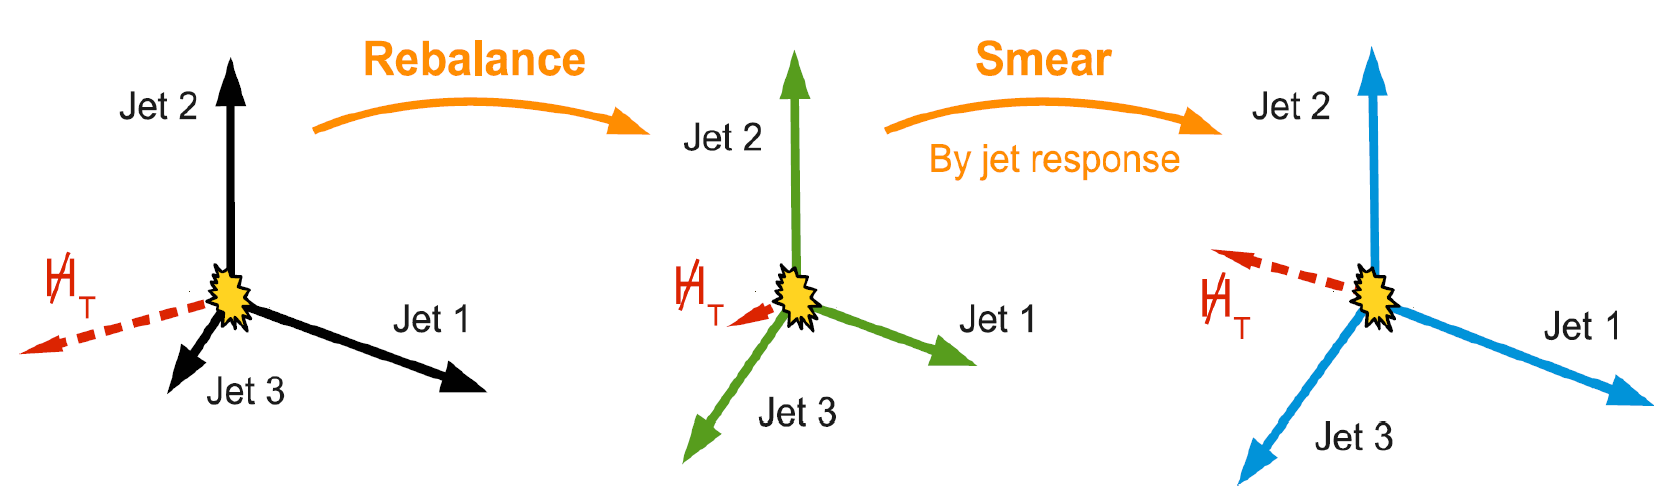
\includegraphics[width=0.90\textwidth]{results/qcd_scetch.png}

\end{tabular}
\end{center}
\caption{This sketch illustrates the Rebalance and Smear method used to estimate the QCD background contribution\cite{AN:2012}.}
\label{fig:qcd_scetch}
\end{figure}
This method involves the following steps:
First, jets with $\pt >15 \gev$ in an event are balanced in the transverse plane, using a kinematic fit. When a prescaled trigger is used to collect the events they have to be smeared $N$ times according to the jet response function \footnote{The jet response function describes the mis-measurement of jets and has been obtained from simulation and has been corrected for the differences to data}, in order to reduce statistical uncertainties.
The non-Gaussian tale of the jet response function are very important for the high \HT and \MHT regions. Much work has been done to model these tails precisely.\\
This procedure is repeated 100 times. The mean and variance of the resulting predictions is calculated and used for the QCD background estimation.\\
The main uncertainties on the QCD background estimation arises from non-closure, the shape of the jet response functions including the Gaussian width, the tails, the heavy flavor contribution, and the effect of pileup on jet measurements. The resulting total uncertainty adds up to $60-70\%$.\\
The QCD method is extremely important since it is dominant for one of the most sensitive search regions (the $\HT >1400$, $\MHT >200$ region).\\
In addition a factorization method has been used for cross checks. Both method lead to comparable results as can be seen in greater detail in the AN \cite{AN:2012}.
\clearpage

\subsection{The $Z$ to invisible background estimation}
\label{sec:z_invi}
The background arising from events including jets and a $Z$-Boson which decays to two neutrinos has been evaluated with two methods\cite{AN:2012}.\\
\begin{figure}[tbhn]
\begin{center}
\begin{tabular}{c}
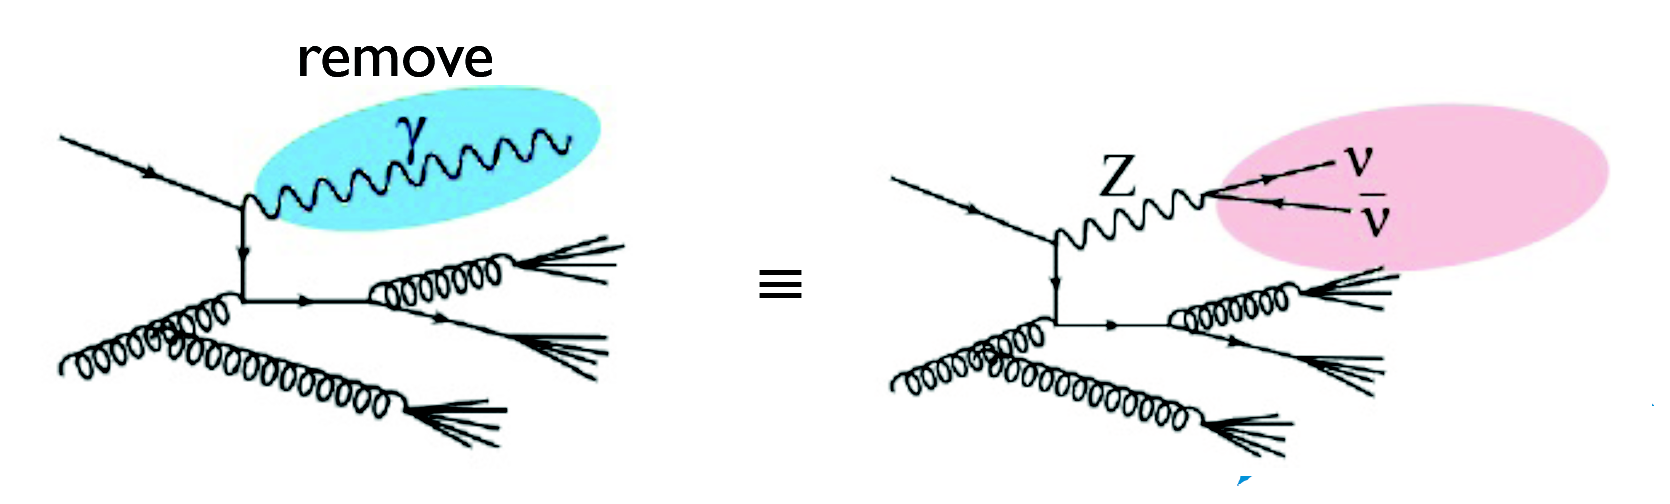
\includegraphics[width=0.90\textwidth]{results/z_photon_scetch.png}

\end{tabular}
\end{center}
\caption{This sketch illustrates the $\gamma$+jets method used for the $Z\rightarrow \nu\nu$ background estimation.}
\label{fig:z_scetch}
\end{figure}
The $Z\rightarrow \nu\nu$ background is estimated by removing the $\gamma$ in a $\gamma$+jets data sample and correcting for the differences between the $\gamma$ and the $Z\rightarrow \nu\nu$ process. 
The $Z$ boson and photon exhibit similar kinematic properties at high boson \pt. Also the hadronic component of these events is similar. %\cite{siehe paper 32-34 ref}.
A $\gamma$+jets sample is corrected for the $\gamma$ reconstruction efficiency and the photon purity. Both are measured from data and the $Z(\nu\bar{\nu})\text{+jets} / \gamma\text{+jets}$ ratio, from simulation, which includes the modeling of the production and acceptance. Fig.~\ref{fig:z_scetch} illustrates the basic idea of removing the $\gamma$ from the sample to model the $\Z\rightarrow\nu\nu$ events.\\
The resulting total correction factor is $0.28\pm0.06$ for the baseline selection. The theoretical uncertainty because of EWK\cite{AN:2012}, leading log on the $\gamma$-Z cross-section ratio of $21-42\%$ is the dominate systematic uncertainty. Also the detector acceptance of $\pm5\%$, the photon reconstruction efficiency and the purity of the photon sample contribute. \\
For a cross check a second method is used, which starts with jets and $Z\rightarrow \mu\mu$ sample. The muons are removed and the branching ratio of $R(Z\rightarrow \nu\nu /Z \rightarrow \mu\mu)$ is applied.\\
The prediction for the baseline selection of $602\pm100$ events agrees well with the $595\pm135$ events predicted from the $\gamma$+jets method. 

\subsection{The hadronic $\tau$ background estimation}
\label{sec:had_tau}
One part of the \ttbar and \wpj events can decay to a $\tau$ further decaying hadronically. This background is estimated by selecting a muon control sample similar to the control sample used for the lost-lepton estimation. Instead of a \HT-\MHT cross trigger an inclusive $\mu$ or a $\mu$ trigger with at least two jets is used with exactly one $\mu$ with $\pt >20\gev$ and $|\eta|<2.1$.\\
The background is estimated by replacing the muon \pt by a jet \pt taken from a simulated response function for a hadronically-decaying $\tau$ which can be seen in Fig.~\ref{fig:hadTau}. The \HT and \MHT distribution is recalculated including the $\tau$-jet, and the search selections are applied to predict the hadronic-$\tau$ background.\\
The $\tau$-jet response template is parametrized in $\pt^{jet} / \pt^{\tau}$ and is obtained from \ttbar and \wpj MC events by matching a reconstructed $\tau$-jet with the corresponding generated $\tau$. In addition corrections have been applied to account for the trigger efficiency, acceptance and efficiency of the $\mu$ selection, and the relative branching ratio of $R(W\rightarrow \tau\nu(\tau\rightarrow hadrons)/(W\rightarrow\mu\nu))=0.69\pm0.05$.\\
The main systematic uncertainties arise from the uncertainty on the correction and additional up to 11\% uncertainty based on non closure and the MC statistics used. In addition systematic uncertainties arise from the $\mu$ acceptance ($\le 13\%$), the $\tau$-jet response function ($\le$ 20\%), and the subtraction of residual QCD multi jet and $Z\rightarrow\mu\mu$ events.\\
\begin{figure}[tbhn]
\begin{center}
\begin{tabular}{c}
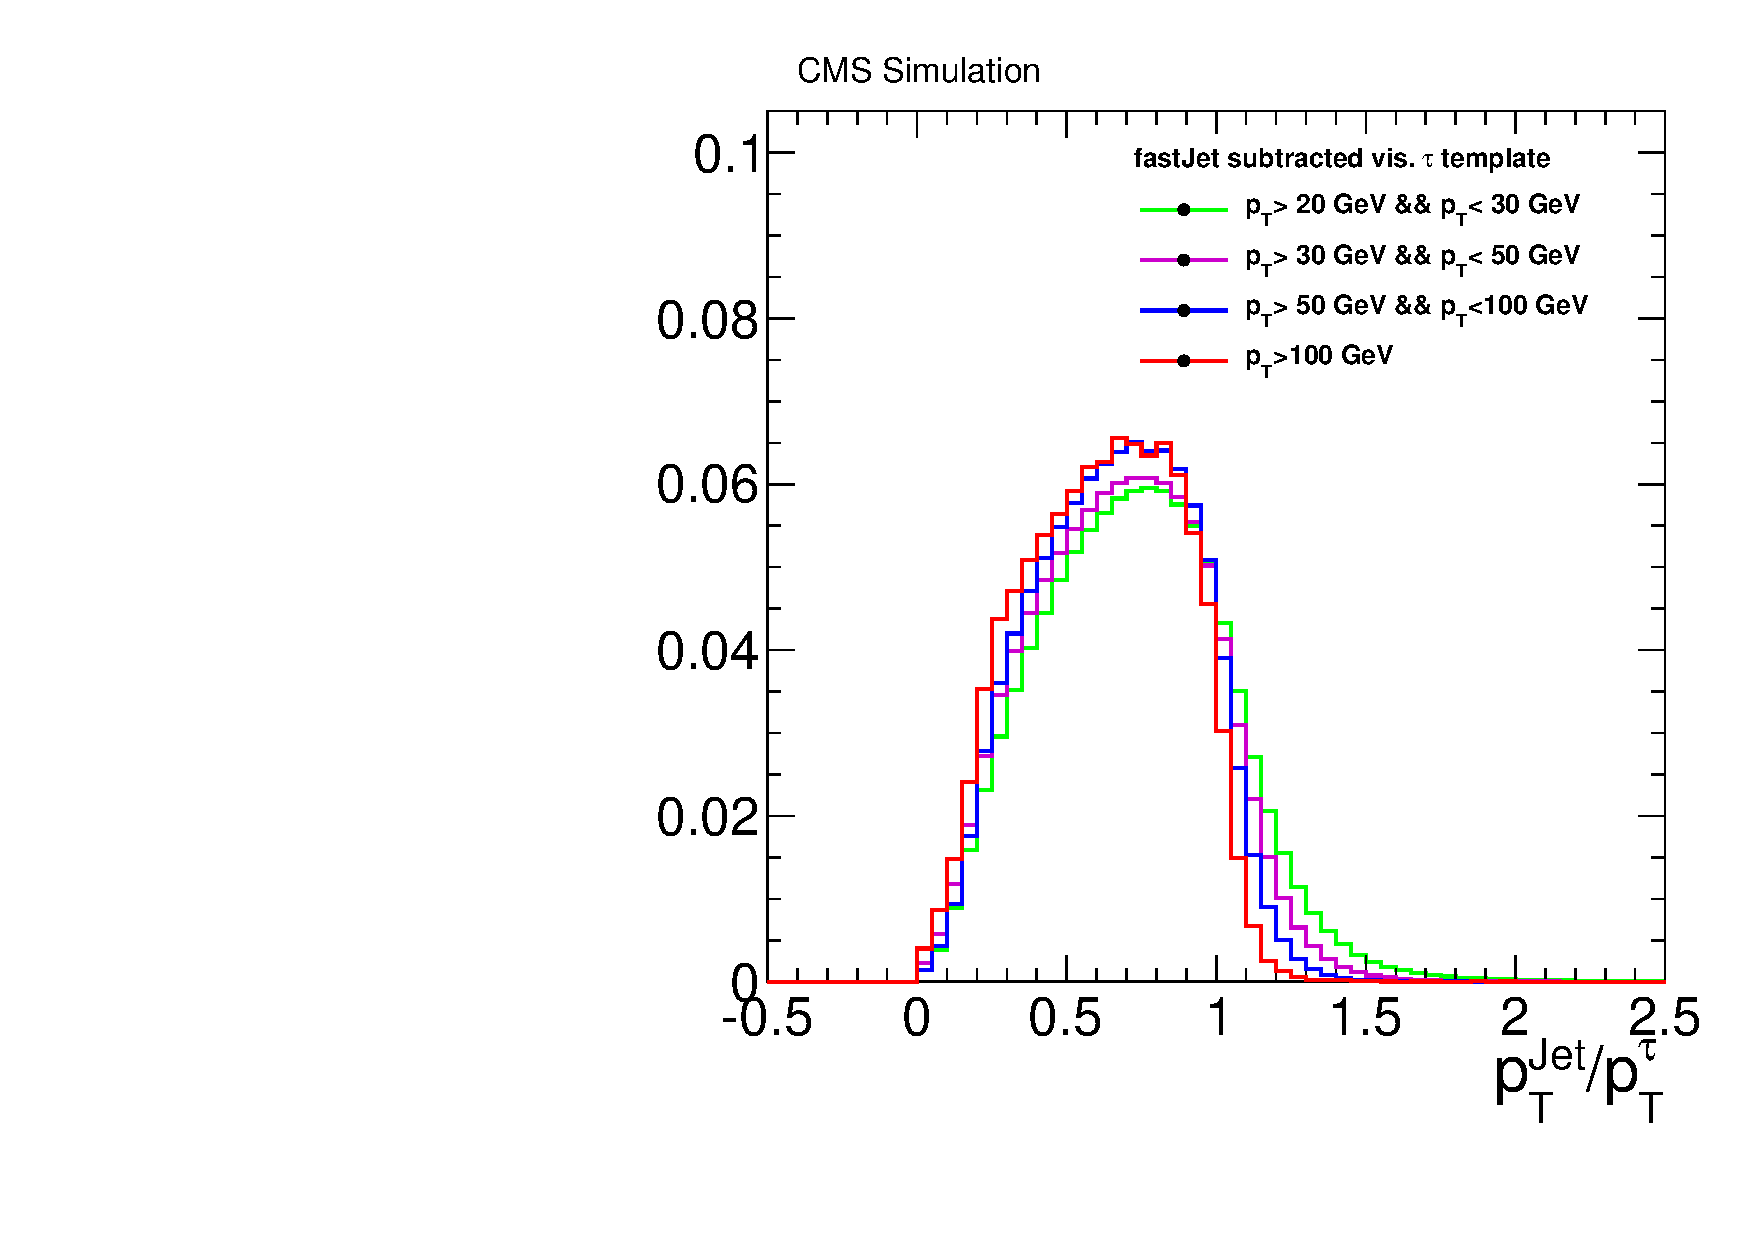
\includegraphics[width=0.60\textwidth]{results/TauTemplate.pdf}

\end{tabular}
\end{center}
\caption{This figure shows a typical hadronic $\tau$ response template used for the background estimation\cite{AN:2012}.}
\label{fig:hadTau}
\end{figure}

\section{Combination of all backgrounds}
\label{sec:combination_bkg}

The combination of all the background estimations and the selection on the full \lumi luminosity can be seen in Tab.~\ref{tab:FinalEventYields}. 
All the background estimations are also shown in Fig.~\ref{fig:htmhtcombined} for the full baseline selection and Fig. ~\ref{fig:summaryHTMHT} for each search region separately. Very good agreement for the \HT and \MHT distribution can be observed. No significant excess above the combined prediction can be observed. This result is interpreted in terms of limits within the cMSSM and Simplified Models in the next section.
\begin{figure}[tbhn]
\begin{center}
%\begin{tabular}{cc}
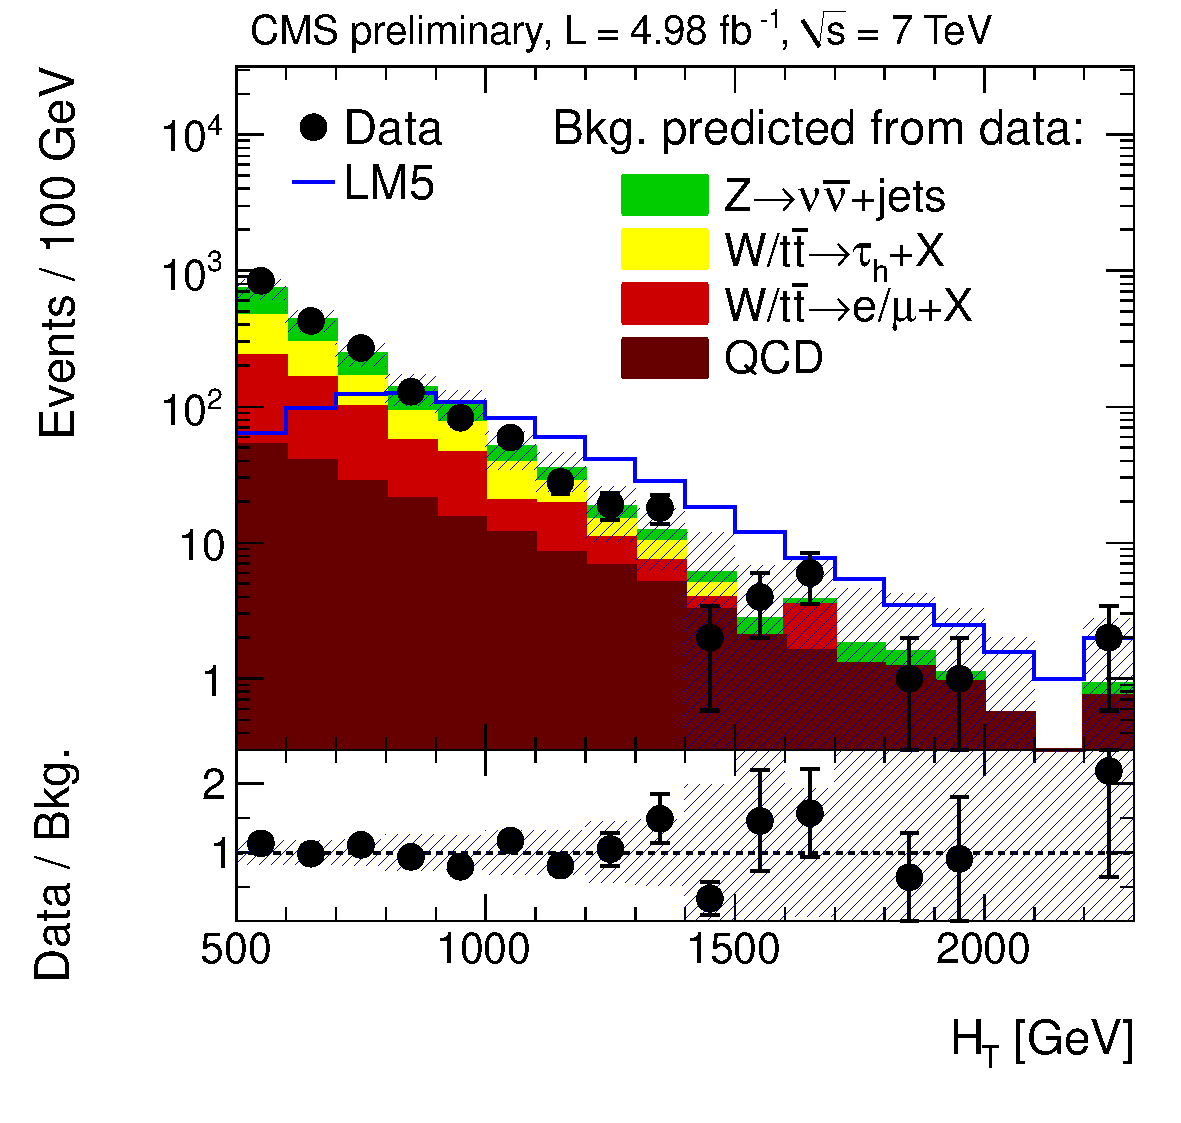
\includegraphics[width=0.45\textwidth]{results/RA2DataVsEstimatedBkg_HT.pdf}
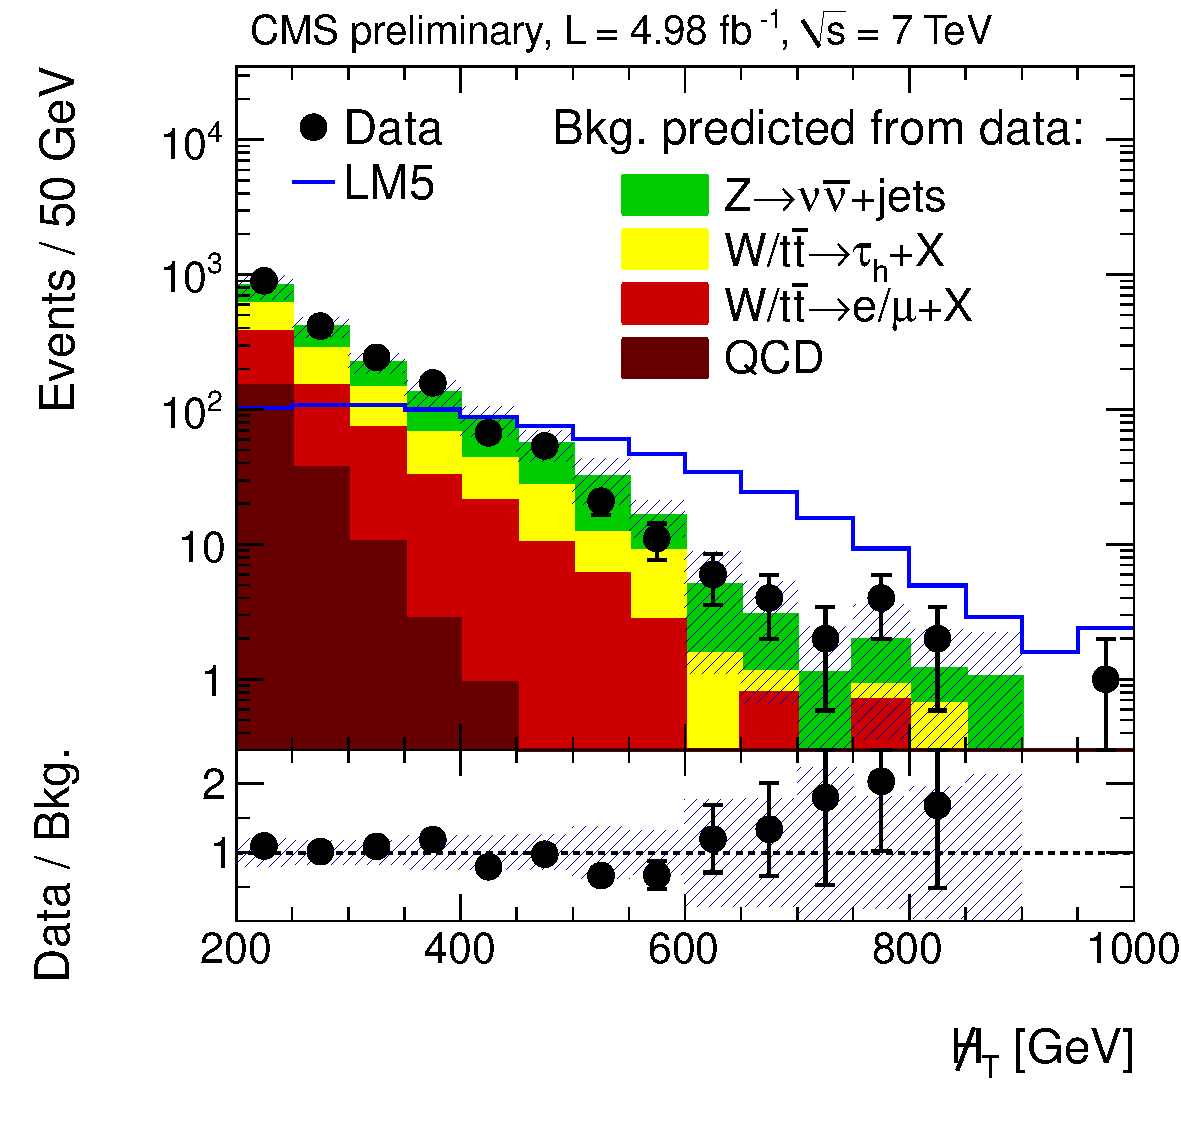
\includegraphics[width=0.45\textwidth]{results/RA2DataVsEstimatedBkg_MHT.pdf}
%\end{tabular}
\end{center}
\caption{\HT (left) and \MHT (right) distributions in data compared to the combined data-driven background predictions and to the SUSY LM5 benchmark scenario.
The ratio of the selection on data to the combined data-driven background predictions can be found on the bottom.
The hatched area represents the combined systematic and statistical uncertainties on the prediction\cite{AN:2012}.
}
%%The bin-by-bin combination of the background contributions and their uncertainties has been performed in a simplified way assuming Gaussian probability distributions.}
\label{fig:htmhtcombined}
\end{figure}


\begin{figure}[tbhn]
\begin{center}
%\begin{tabular}{cc}
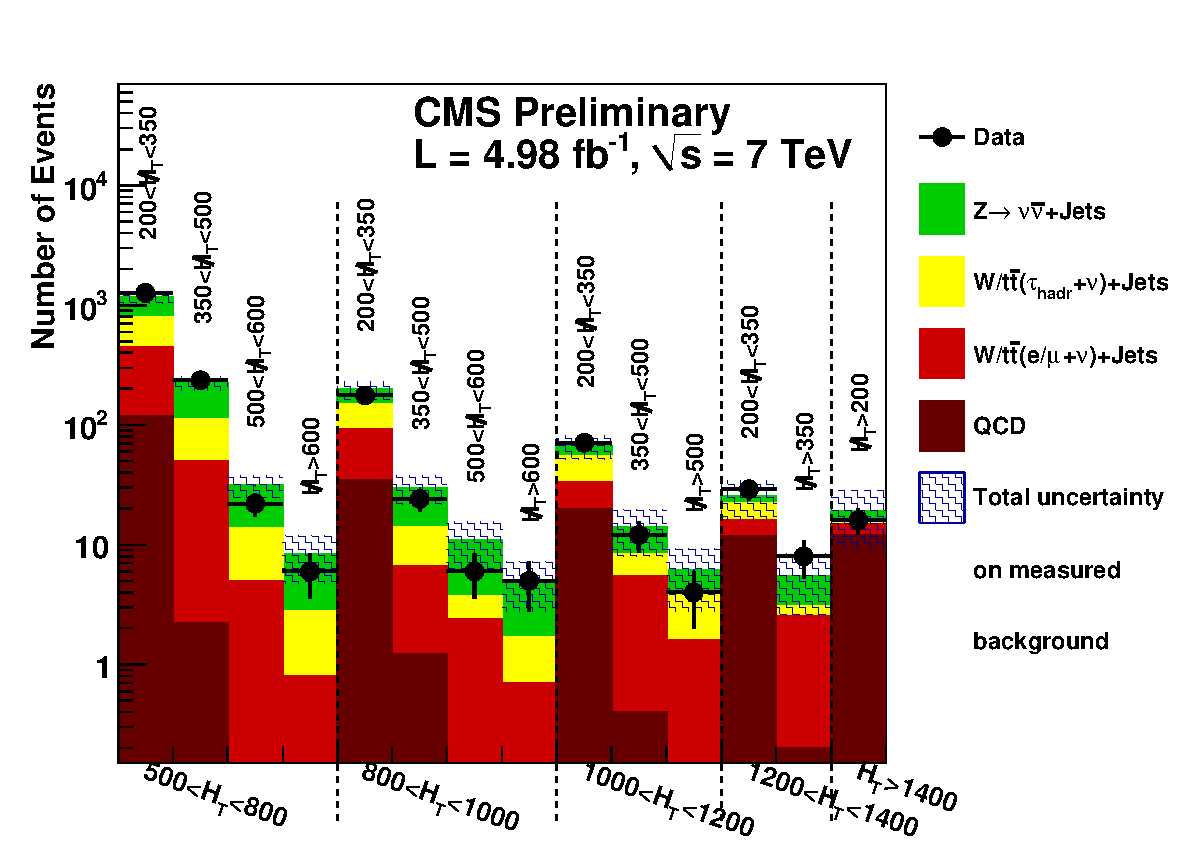
\includegraphics[width=0.85\textwidth]{results/c_RA2ResultSummaryHTMHT.pdf}
%\end{tabular}
\end{center}
\caption{Summary of backgrounds estimated from data and observed events in data for 14 search regions used in the analysis and presented in Tab.~\ref{tab:FinalEventYields}\cite{AN:2012}}.
%%The bin-by-bin combination of the background contributions and their uncertainties has been performed in a simplified way assuming Gaussian probability distributions.}
\label{fig:summaryHTMHT}
\end{figure}

%In addition the predicted event yields with each total uncertainty from all the different data-driven background estimation methods discussed in the sec. \ref{sec:analyse} and the number of selected events observed in the \lumi are summarized in Tab. ~\ref{tab:FinalEventYields} for all different search bins along with the baseline selection.\\



\begin{sidewaystable}[hbt]
\fontsize{8 pt}{1.0 em}
\selectfont
\begin{center}
\caption{Predicted event yields from the different background estimation methods for the baseline
selection and for the search selections using \lumi dataset. An additional row with
total is added where statistical uncertainties are treated uncorrelated and systematic uncertainties
are added assuming full correlation.
%\todo{this explanation needs modification.} The background combination is performed by taking into account the shape of the uncertainties, and thus the total of each background prediction does not necessarily correspond to the combined background prediction.}
}
\label{tab:FinalEventYields}
{
\begin{tabular}{|rr|rl|rl|rl|rl|rl|r|}
\hline

\multicolumn{2}{|c|}{Selection}
            & \multicolumn{2}{c|}{$z\nu\nu$} 
            & \multicolumn{2}{c|}{$\ttbar/\W$}
            & \multicolumn{2}{c|}{$\ttbar/\W$} 
	    & \multicolumn{2}{c|}{QCD}
            & \multicolumn{2}{c|}{Total }
	    & \multicolumn{1}{c|}{Observed}          \\

HT &MHT     & \multicolumn{2}{c|}{from $\gamma+$jets} 
	    & \multicolumn{2}{c|}{$\to \e,\mu+$X}
            & \multicolumn{2}{c|}{$\to \tau_{\mbox{\tiny hadr}}+$X}  
	    & \multicolumn{2}{c|}{}
            & \multicolumn{2}{c|}{background}  
	    & \multicolumn{1}{c|}{ in data}  \\ 

%%\hline

% updated April 04, 2012 (updating systematics for tauhad)
\hline
500-800    &200-350  & 359.2 &$\pm$ 82.2    & 326.5  &$\pm$ 47.0    &  348.5 &$\pm$ 40.1    & 118.6  &$\pm$ 76.9    & 1152.9 &$\pm$ 128.4   & 1269 \\
500-800    &350-500  & 112.3 &$\pm$ 27.4    &  47.8  &$\pm$  9.2    &   62.5 &$\pm$  8.7    &   2.2  &$\pm$  2.2    &  224.8 &$\pm$  30.3   &  236 \\
500-800    &500-600  &  17.6 &$\pm$  5.6    &   5.0  &$\pm$  2.2    &    8.7 &$\pm$  2.5    &   0.0  &$\pm$  0.1    &   31.3 &$\pm$   6.5   &   22 \\
500-800    &$>$600   &   5.5 &$\pm$  3.1    &   0.8  &$\pm$  0.8    &    2.0 &$\pm$  1.8    &   0.0  &$\pm$  0.0    &    8.3 &$\pm$   3.6   &    6 \\
\hline
800-1000   &200-350  &  48.4 &$\pm$ 19.1    &  57.7  &$\pm$ 15.3    &   56.3 &$\pm$  8.3    &  34.6  &$\pm$ 24.0    &  197.0 &$\pm$  35.3   &  177 \\
800-1000   &350-500  &  16.0 &$\pm$  7.3    &   5.4  &$\pm$  2.3    &    7.2 &$\pm$  2.0    &   1.2  &$\pm$  1.3    &   29.8 &$\pm$   8.0   &   24 \\
800-1000   &500-600  &   7.1 &$\pm$  4.5    &   2.4  &$\pm$  1.5    &    1.3 &$\pm$  0.6    &   0.0  &$\pm$  0.2    &   10.8 &$\pm$   4.8   &    6 \\
800-1000   &$>$600   &   3.3 &$\pm$  2.0    &   0.7  &$\pm$  0.7    &    1.0 &$\pm$  0.3    &   0.0  &$\pm$  0.1    &    5.0 &$\pm$   2.2   &    5 \\
\hline
1000-1200  &200-350  &  10.9 &$\pm$  5.5    &  13.7  &$\pm$  3.8    &   21.9 &$\pm$  4.6    &  19.7  &$\pm$ 13.3    &   66.2 &$\pm$  15.5   &   71 \\
1000-1200  &350-500  &   5.5 &$\pm$  3.5    &   5.0  &$\pm$  4.4    &    2.9 &$\pm$  1.3    &   0.4  &$\pm$  0.7    &   13.7 &$\pm$   5.8   &   12 \\
1000-1200  &$>$500   &   2.2 &$\pm$  2.9    &   1.6  &$\pm$  1.2    &    2.3 &$\pm$  1.0    &   0.0  &$\pm$  0.2    &    6.1 &$\pm$   3.3   &    4 \\
\hline
1200-1400  &200-350  &   3.1 &$\pm$  2.0    &   4.2  &$\pm$  2.1    &    6.2 &$\pm$  1.8    &  11.7  &$\pm$  8.3    &   25.1 &$\pm$   9.0   &   29 \\
1200-1400  &$>$350   &   2.3 &$\pm$  2.3    &   2.3  &$\pm$  1.4    &    0.6 &$\pm$  0.8    &   0.2  &$\pm$  0.6    &    5.5 &$\pm$   2.9   &    8 \\
\hline
$>$1400    &$>$200   &   3.2 &$\pm$  2.4    &   2.7  &$\pm$  1.6    &    1.1 &$\pm$  0.5    &  12.0  &$\pm$  9.1    &   18.9 &$\pm$   9.6   &   16 \\
\hline
Baseline      &         & 596.6 &$\pm$ 165.0   & 475.8  &$\pm$ 76.2    &  522.4 &$\pm$ 67.0    & 200.7  &$\pm$ 82.7    & 1795.4 &$\pm$ 205.9   & 1885 \\
\hline

\end{tabular}
}
\end{center}


\end{sidewaystable}




%From the fig.\ref{fig:summaryHTMHT} and tab.\ref{tab:FinalEventYields} one can observe consistency of data and SM background estimation only. This lack of a signal is interpreted in the following section for the cMSSM and simplified models.









\clearpage


\section{Interpretation of the results}
\label{sec:interpretation}

The results are interpreted by setting limits with a $95\%$ confidence level (CL) with the CLs method\cite{0954-3899-28-10-313}\cite{Thomas1999435} within the cMSSM and simplified models.\\
The CLs is a ratio of confidence levels $CL_s = \frac{CL_{s+b}}{CL_b}$\footnote{ where $CL_{s+b}$ is the confidence in the signal+background hypothesis, and
$CL_b$ is the confidence in the background-only hypothesis.} designed to obtain the best limits while avoiding excluding signals, to which the analysis is not really sensitive to.
The confidence in a specific hypothesis $x$ is given by the probability that the test-statistic $Q$ being the likelihood ratio \cite{CMS-PAS-SUS-11-004} is less than or equal to the observed value in the data
$Q_{obs}$:
\begin{equation}
CL_x = P_x(Q\leq Q_{obs}).
\label{eq:sec7:clx}
\end{equation}
Each of the $14$ bins in \HT and \MHT as summarized in Tab.~\ref{tab:FinalEventYields} are used as statistically independent channels in the limit calculation. The used test-statistic $Q$ is constructed using the product of the individual likelihoods per channel. The correlation of the systematic uncertainties among different bins is taken into account. Especially the similarity of the isolated muon control sample used for the lost-lepton and for the hadronic-tau
background estimation methods are taken as correlated into account.\\
\subsection{Interpretation within the cMSSM}
\label{sec:cMSSM}
As discussed in Sec.~\ref{sec:msugra} the CMSSM has only five independent parameters. The signal cross section is calculated at NLO using PROSPINO \cite{Beenakker:1996ed}. For the LM5 \footnote{$m_{0}=230\gev,m_{1/2}=360\gev,A_{0}= 0,tan\beta = 10, \text{and } sign(\mu) > 0$} benchmark point the \HT and \MHT signal are shown in Fig.~\ref{fig:htmhtcombined}.\\
The limits are calculated for the $m_{0},m_{1/2}$ plane and are translated to the $m_{g},m_{q}$ plane while the other parameters are fixed to $A_{0}= 0,tan\beta = 10, \text{ and  sign}(\mu) > 0$.\\
From cMSSM signal samples the efficiency of the event selection for each different parameter set of $m_{0},m_{1/2}$ is evaluated. This expected event selection efficiency is used to set limits with the $CL_s$ method.\\
The uncertainty on the efficiency of the event selection takes the statistical component, the jet energy scale, the jet energy resolution, PDF uncertainties, the uncertainty on the luminosity, trigger inefficiency and inefficiency due to event cleaning into account.
Fig.~\ref{fig:cMSSM_limit} shows the observed limit together with the expected and the $\pm$~1 sigma uncertainty band for the $m_{0},m_{1/2}$ and for the $m_{g},m_{q}$. The dashed line with the yellow band shows the expected limit together with the $\pm 1$~ sigma uncertainty band. Everything below the observed limit is excluded at 95\% confidence level. For comparison the limit obtained with the same methods on data from 2010 corresponding to 36$pb^{-1}$ are shown. The increased statistics lead to a much larger excluded region.

\begin{figure}[tbhn]
\begin{center}
\begin{tabular}{c}
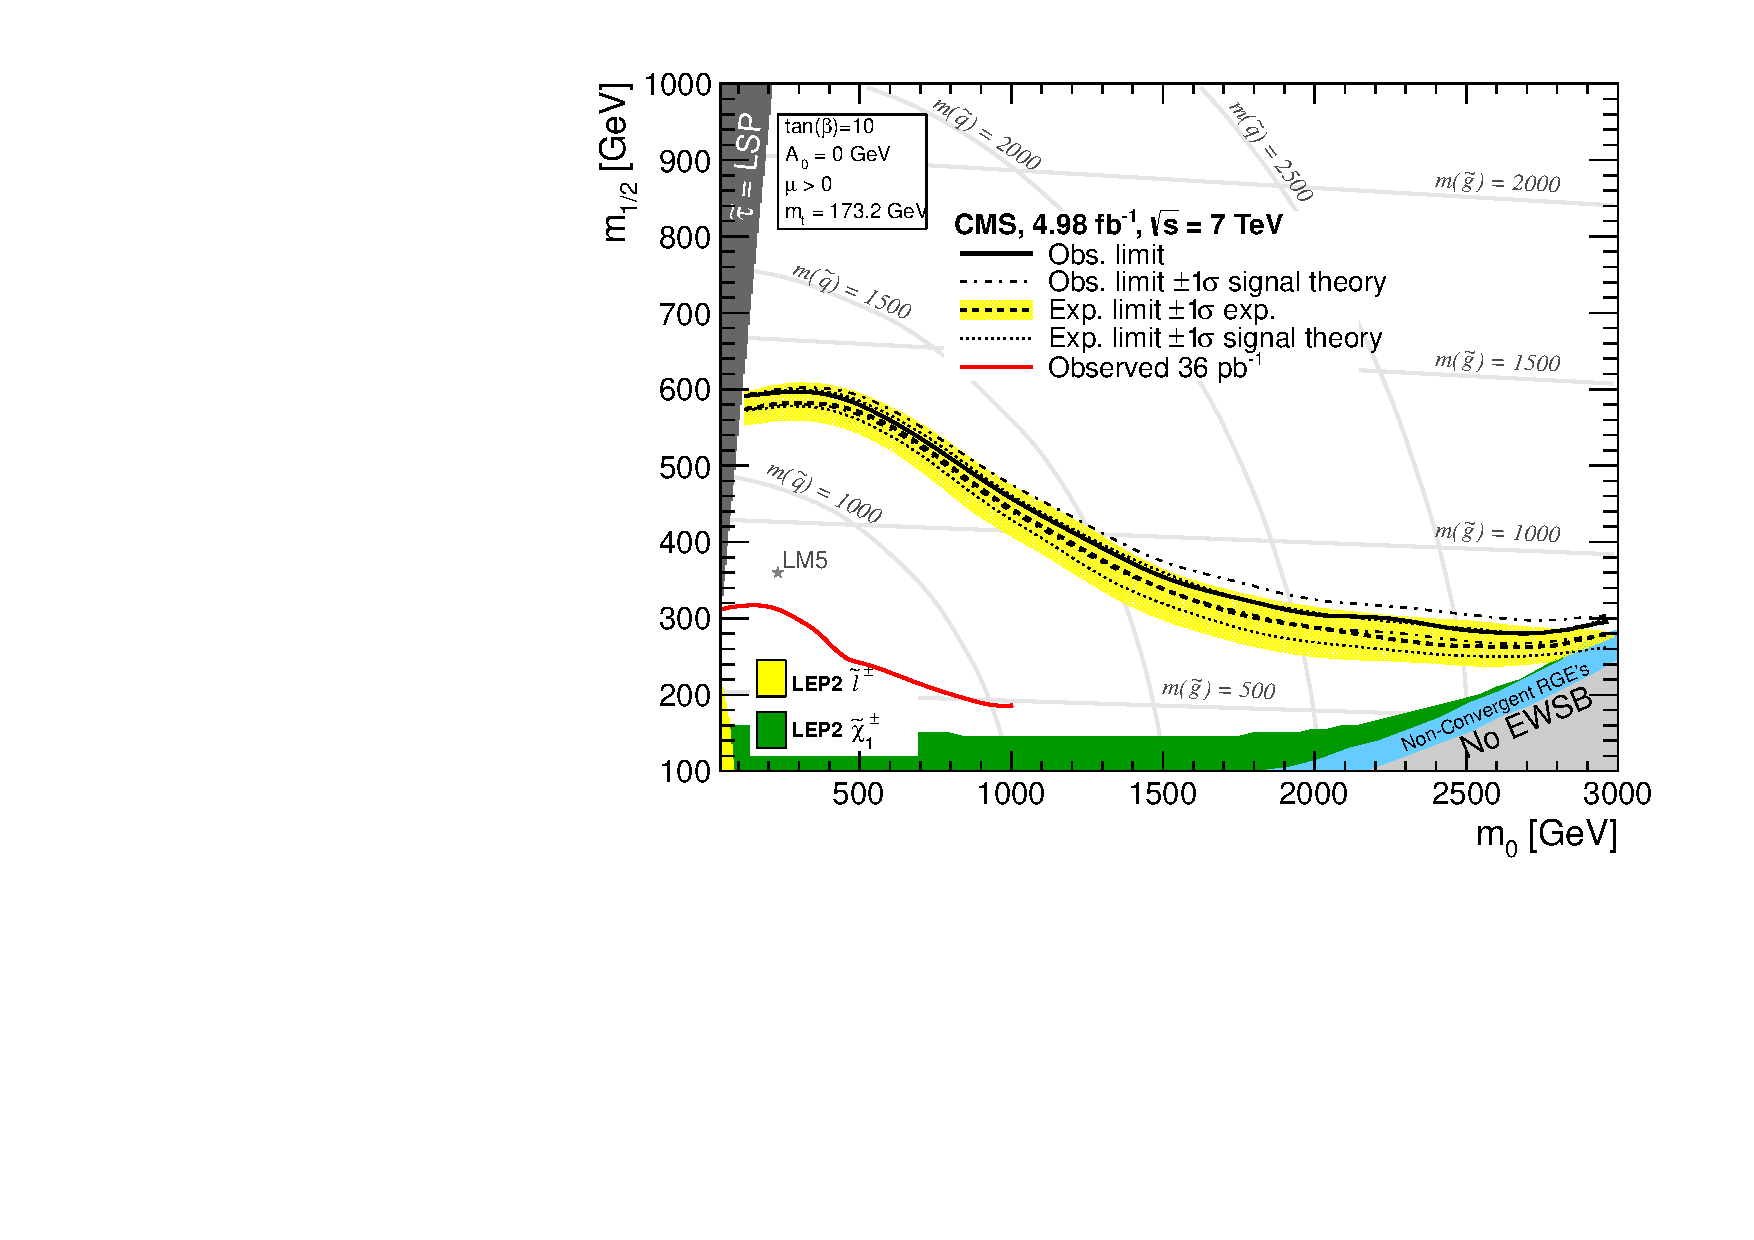
\includegraphics[width=0.85\textwidth]{results/cMSSM_Mzero_Mhalf_Exclusion_.pdf}\\
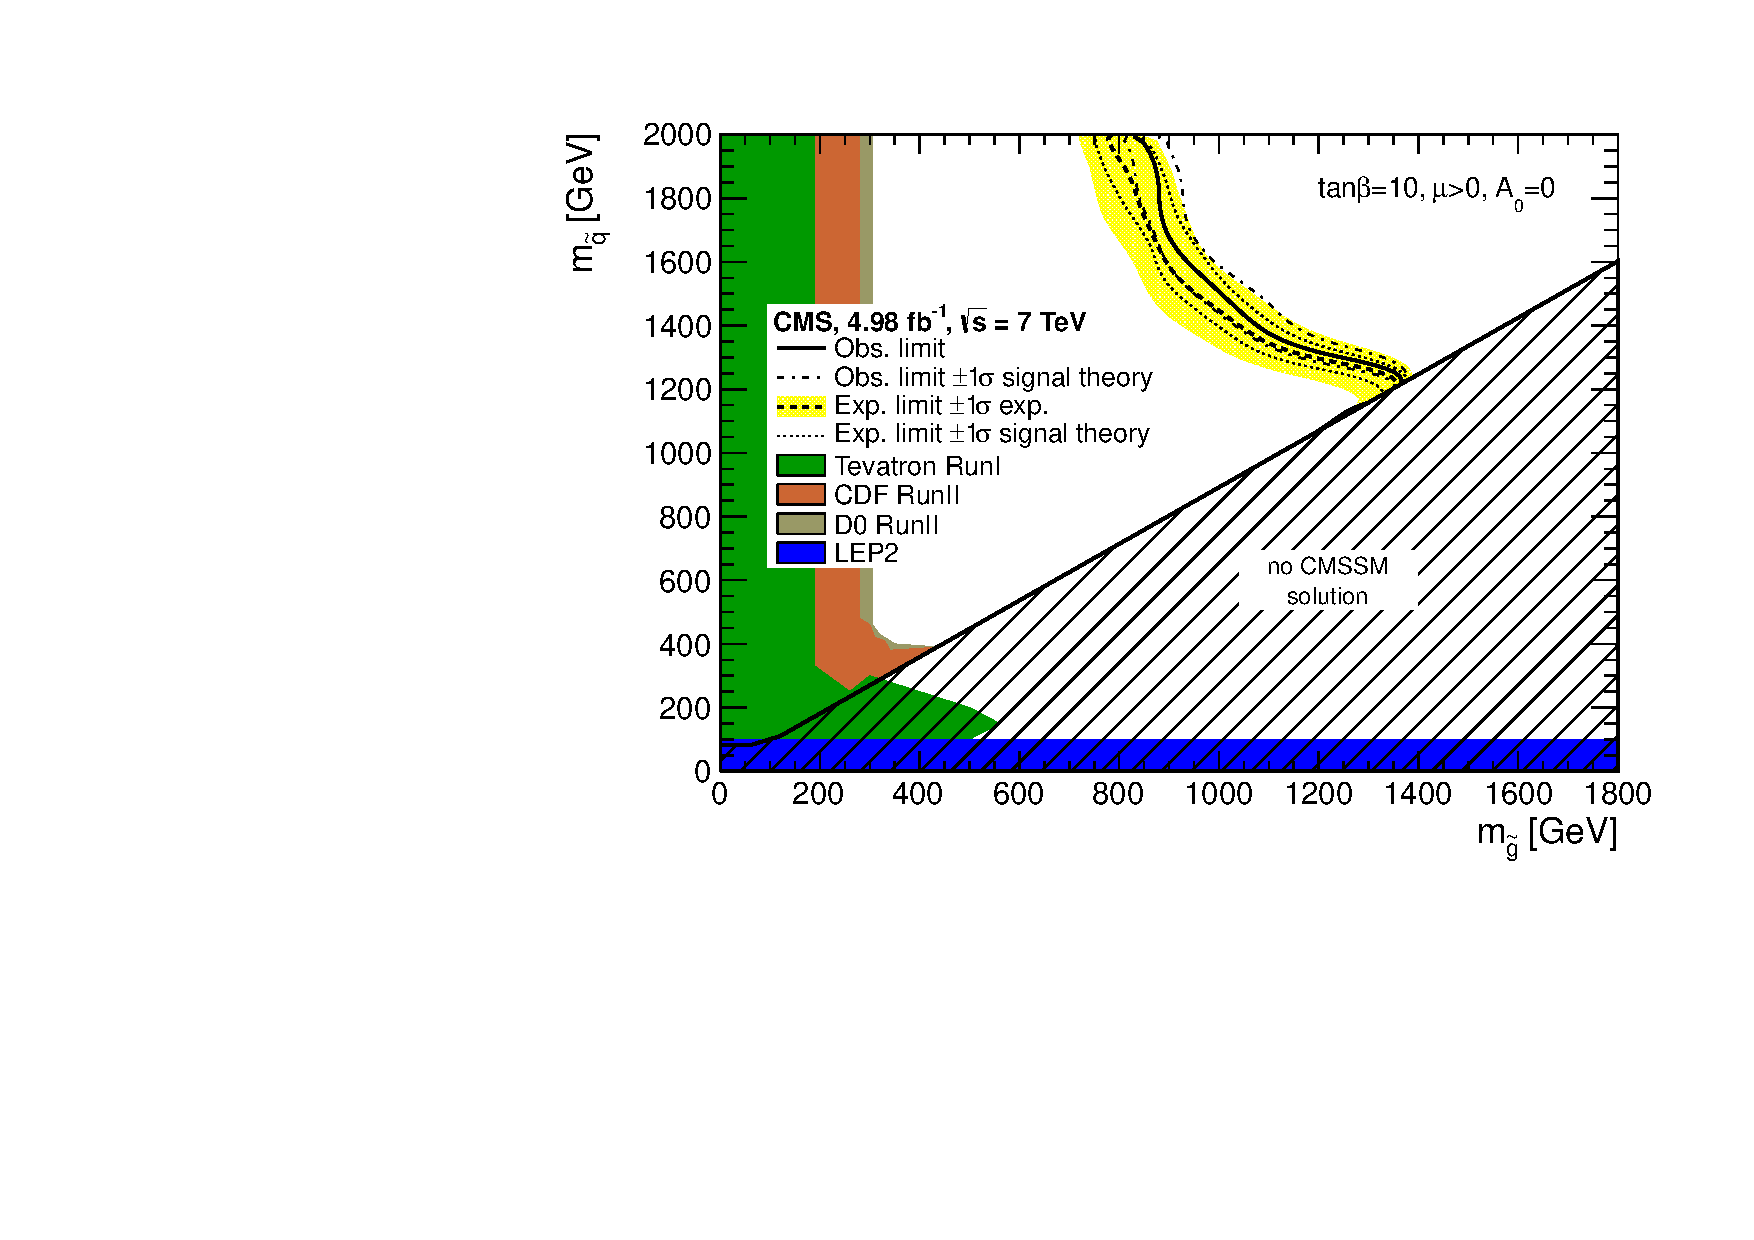
\includegraphics[width=0.85\textwidth]{results/cMSSM_MGluino_MSquark_Exclusion_.pdf}
\end{tabular}
\end{center}
\caption{Both plots shows the interpretation of the results within the cMSSM model for the $m_{0},m_{1/2}$ plane on top and the same limits translated to the $m_{\tilde g},m_{\tilde q}$ plane on bottom. Everything below the observed limit (black line) is excluded at 95\% CL. The dashed line with the yellow band shows the expected limit together with the $\pm 1$~ sigma uncertainty band.
}
%%The bin-by-bin combination of the background contributions and their uncertainties has been performed in a simplified way assuming Gaussian probability distributions.}
\label{fig:cMSSM_limit}
\end{figure}
\clearpage

\subsection{Interpretation with Simplified Model Spectra}
\label{sec:simplified}
The results of the analysis are also interpreted within the Simplified Model Spectra (SMS).\\
The results are interpreted in two benchmark simplified models:
\begin{itemize}
 \item pair-produced gluinos, where each gluino decays directly to two lighter quarks and the LSP
 \item pair-produced squarks, where each squark decays to one gluon or quark and the LSP 
\end{itemize}
In Fig.~\ref{fig:diagram} the respective diagrams for these simplified models are presented.
\begin{figure}[tbhn]
  \begin{center}
      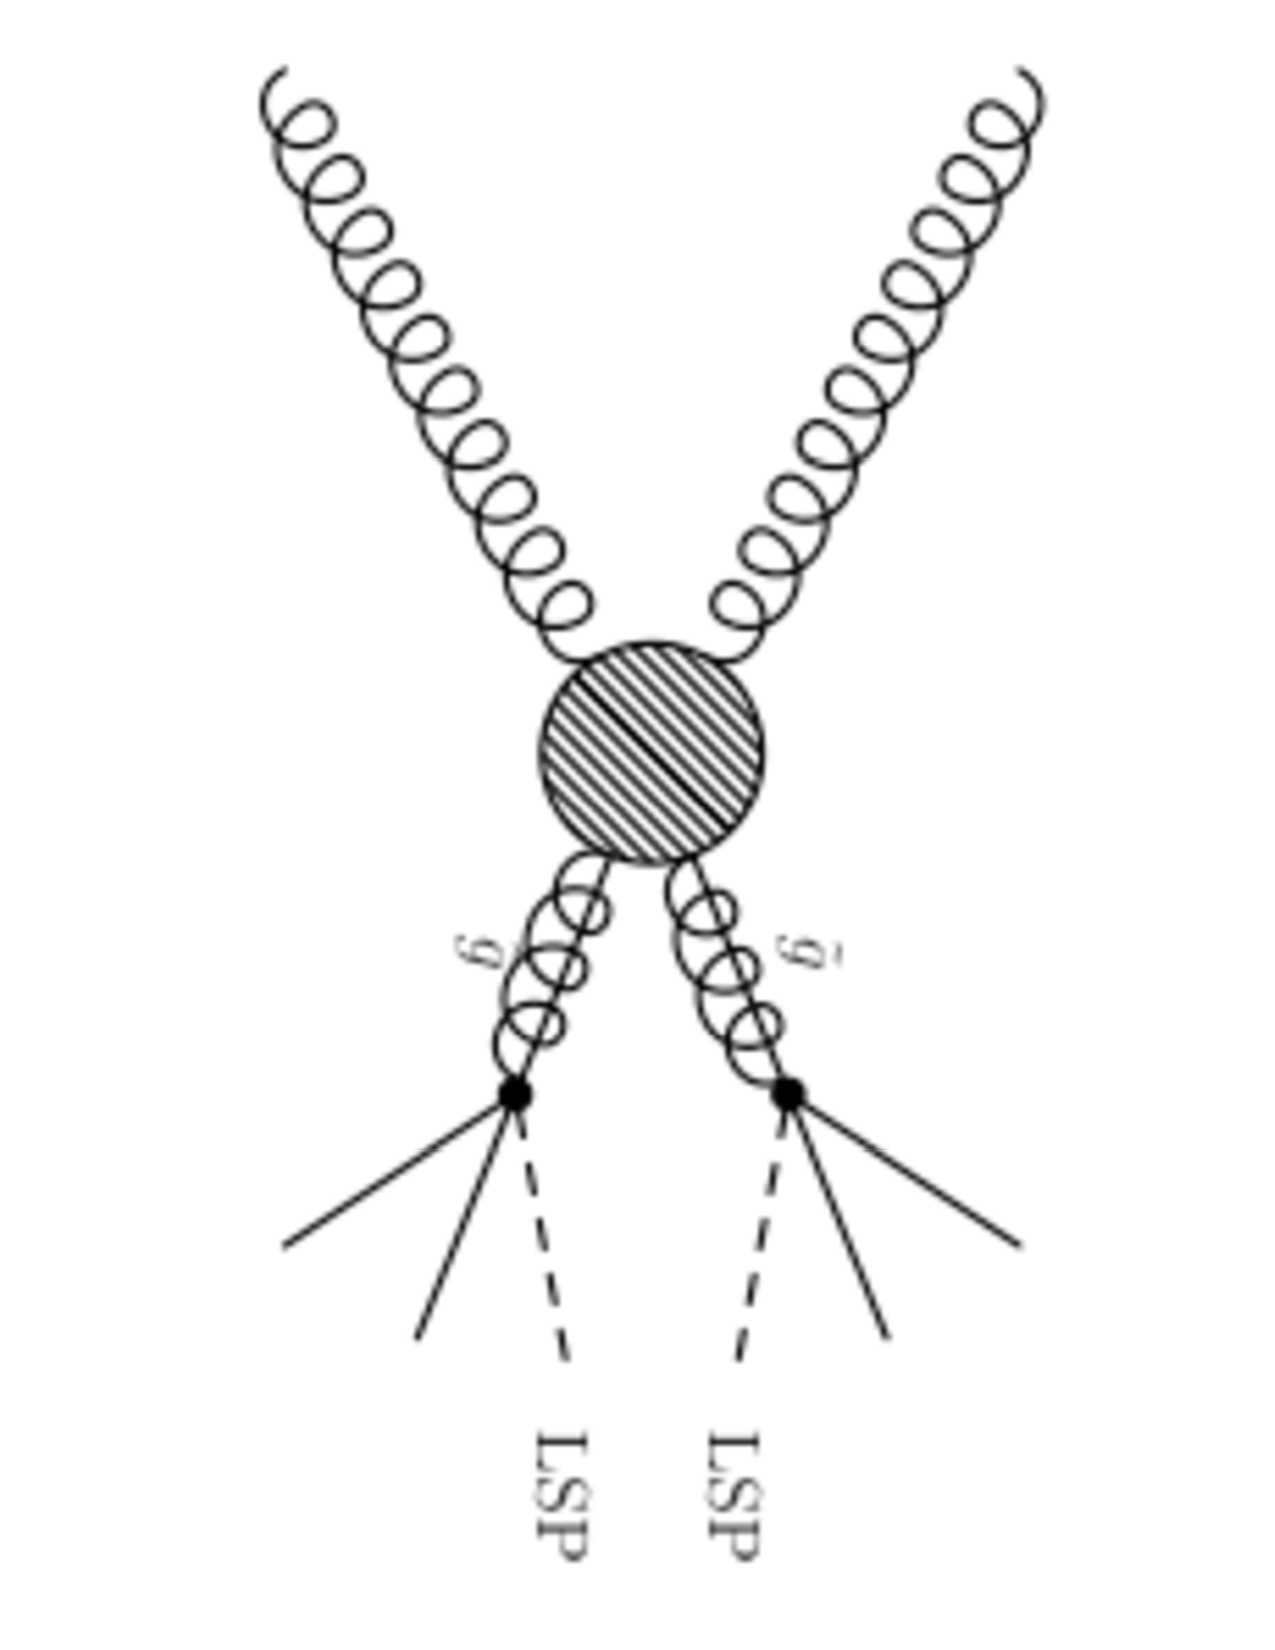
\includegraphics[angle=90,width=0.4\textwidth]{results/T1.pdf}
      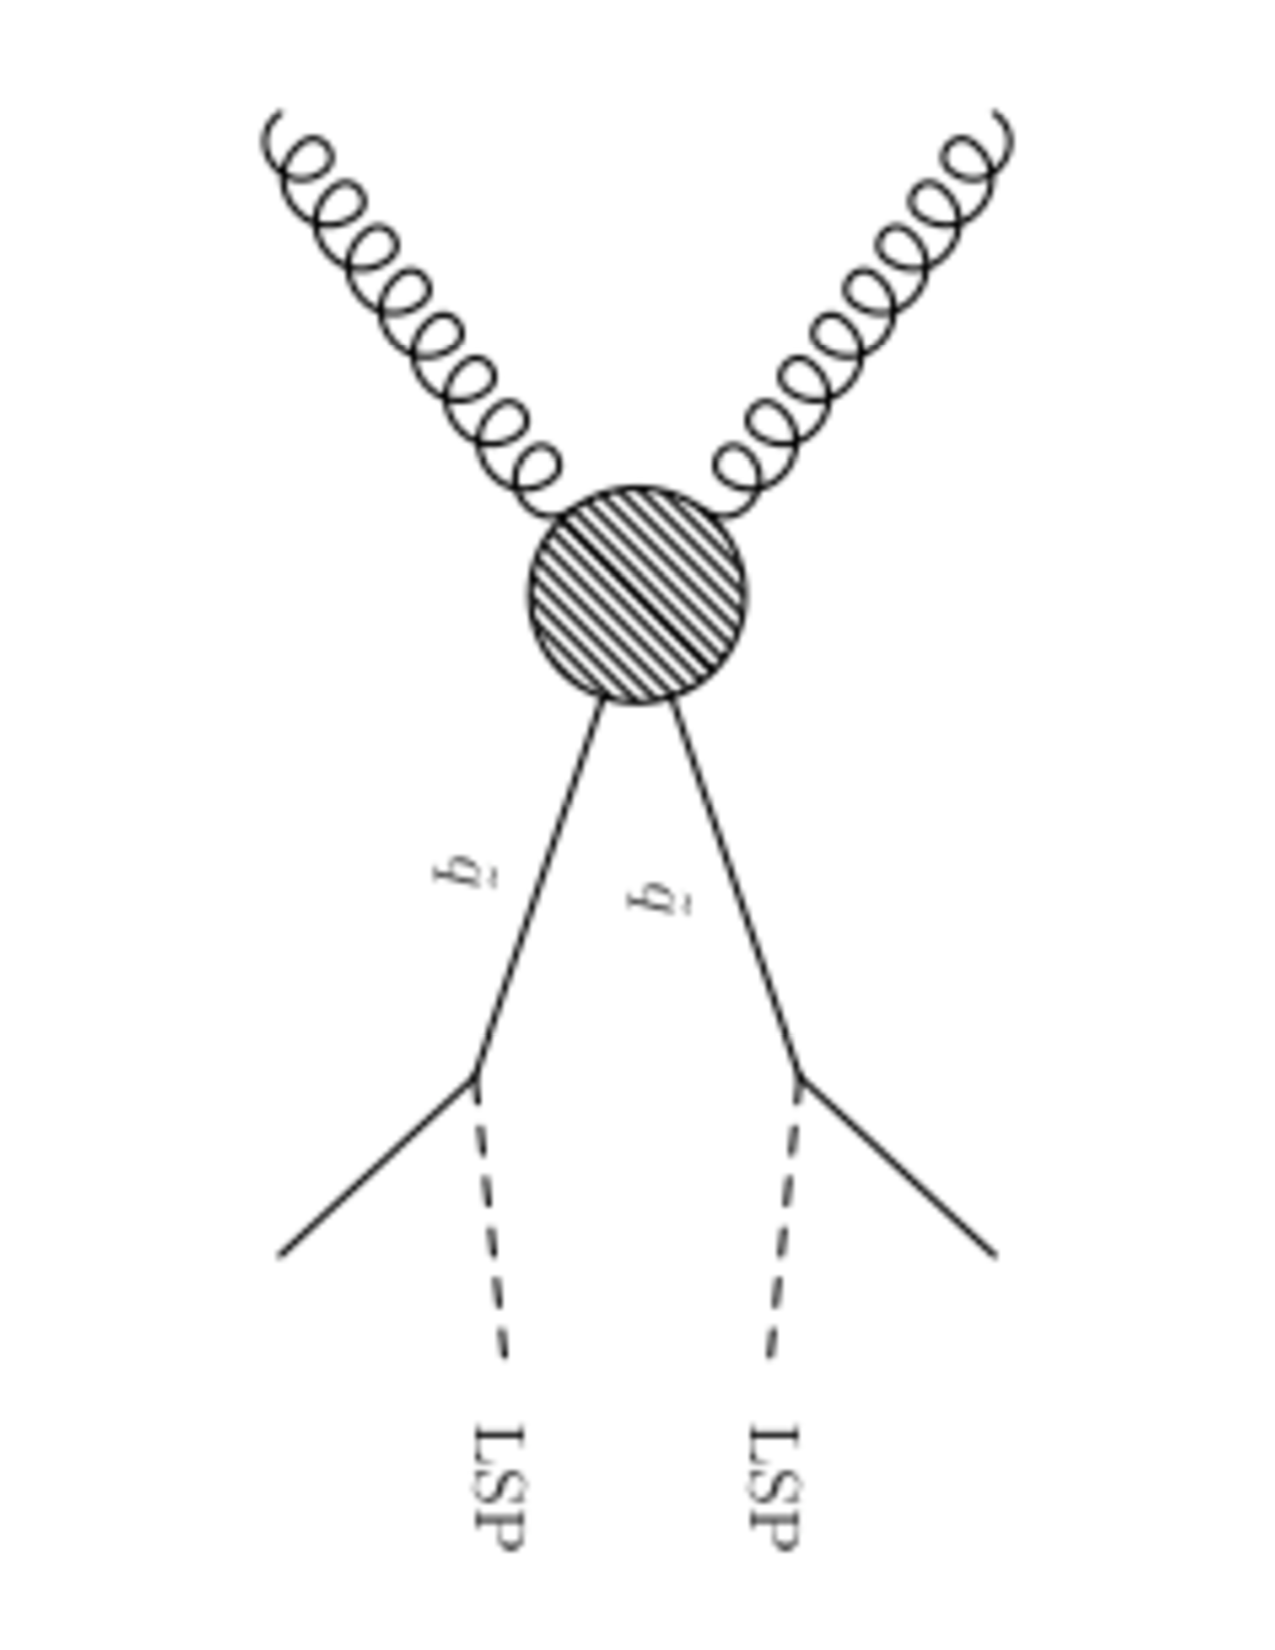
\includegraphics[angle=90,width=0.4\textwidth]{results/T2.pdf}\\[-5mm]
%      \includegraphics[angle=90,width=0.3\textwidth]{limitssms_figures/T3.pdf}
%      \includegraphics[angle=90,width=0.3\textwidth]{limitssms_figures/T4.pdf}
        \caption{Feynman diagram of simplified models. Left: gluino pair production; right: squark pair production.}
        %; bottom row: one single-step cascade decay for gluino pair production and squark pair production.}
    \label{fig:diagram}
  \end{center}
\end{figure}
The role of simplified models is to represent observable processes. Several
topologies are chosen that can bracket the kinematics of the different final states.
For each topology several masses are generated for each of the particles
involved. This way more mass splittings can be explored than in the cMSSM where
the ratio of the gluino and the LSP masses is approximately fixed. 
%Cross sections calculated with Prospino~\cite{Beenakker:1996ed} are assumed further. 
In the case of limit derivation, it is useful to have a reference cross section to
compare results between analyses and experiments.\\
The cross-section limits for the gluino pair production (topology T1) and 
squark pair production (topology T2) are shown in
Fig.~\ref{fig:limitsT1T2}.


\begin{figure}[tbhn]
  \begin{center}
    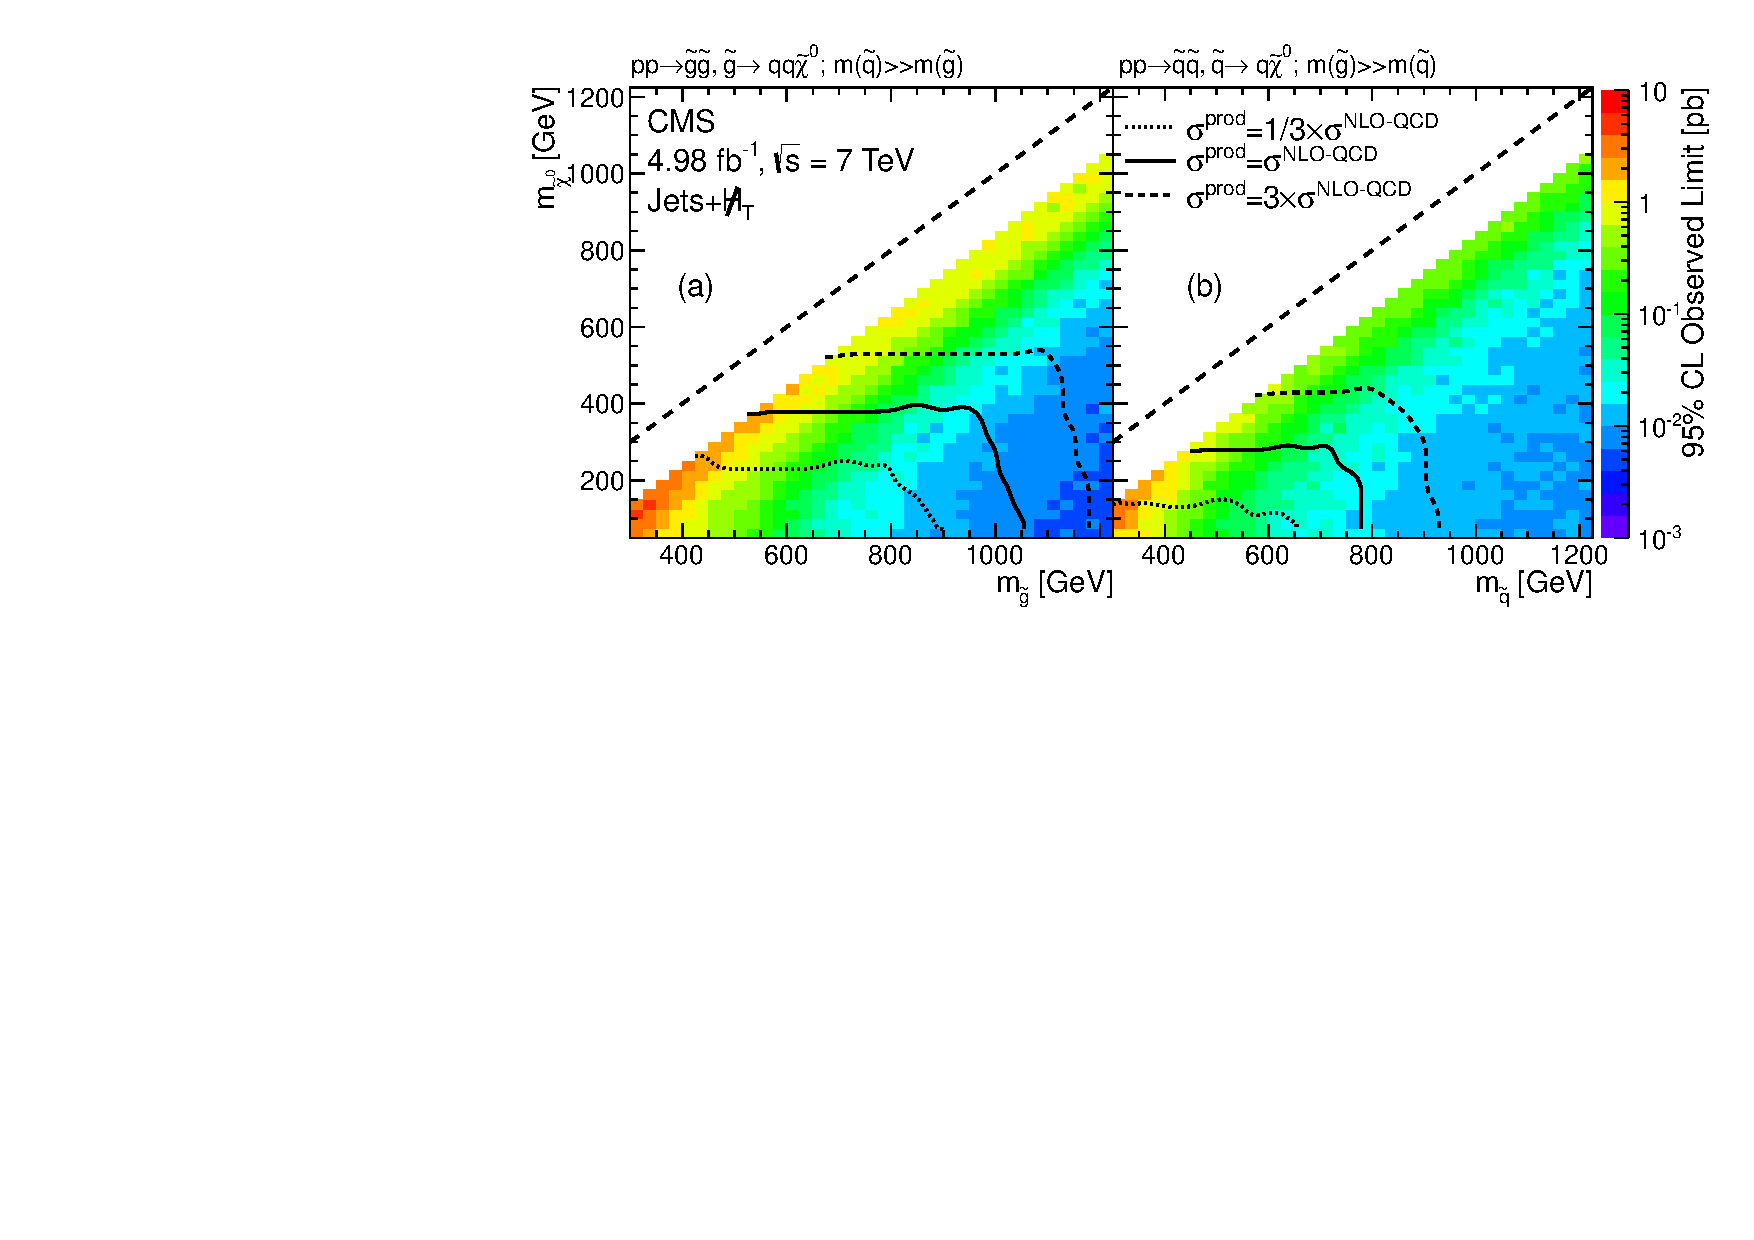
\includegraphics[width=0.80\textwidth]{results/T1T2_combined_ObsLimit_mMother_mLSP.pdf}
    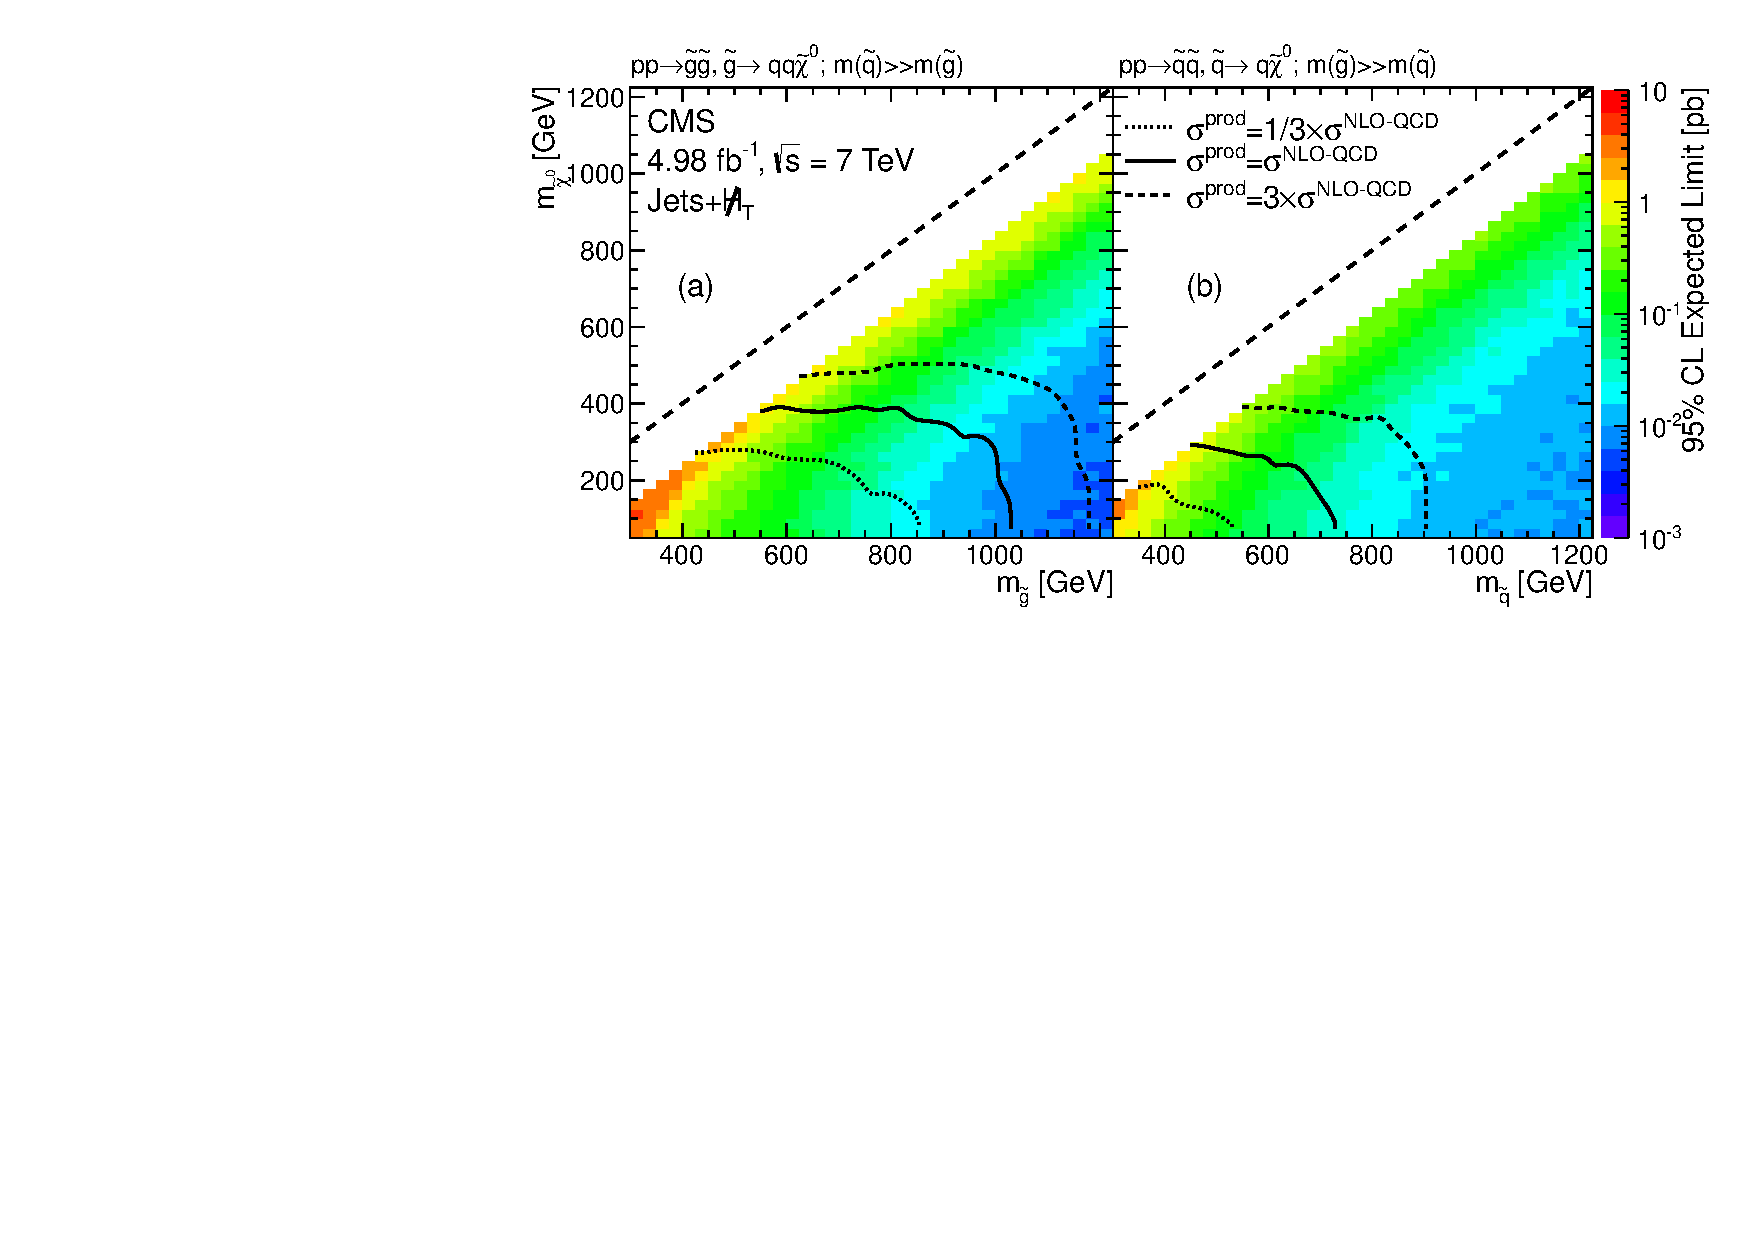
\includegraphics[width=0.80\textwidth]{results/T1T2_combined_ExpLimit_mMother_mLSP.pdf}
    \caption{(Top) {\bf Observed} and (Bottom) {\bf Expected} {\bf 95\% C.L. exclusion limits} for the 
    (a) gluino pair production (topology T1), and
    (b) squark pair production (topology T2).}
    \label{fig:limitsT1T2}
  \end{center}
\end{figure}

